\section{Introduction}
\label{sec:introduction}

Deep neural networks are vulnerable to adversarial examples: imperceptible perturbations that cause confident misclassifications~\citep{szegedy2014intriguingpropertiesneuralnetworks, goodfellow2015explainingharnessingadversarialexamples}. This vulnerability poses serious risks in safety-critical settings such as autonomous driving and medical diagnosis, where a single misclassification can have catastrophic consequences. Adversarial training~\citep{madry2019deeplearningmodelsresistant} remains the dominant defense, and substantial progress has been tracked through standardized benchmarks like RobustBench~\citep{croce2021robustbenchstandardizedadversarialrobustness}, which ranks models by their accuracy under the AutoAttack ensemble~\citep{croce2020reliableevaluationadversarialrobustness}. Yet a fundamental tension exists between robustness and standard accuracy~\citep{tsipras2019robustnessoddsaccuracy}, and recent work on certified defenses~\citep{cohen2019certifiedadversarialrobustnessrandomized} has shifted attention toward provable guarantees rather than empirical attack evaluations alone.

A critical limitation of current evaluation practice is that robustness is almost always reported as a single aggregate number. Whether the metric is empirical robust accuracy or a certified lower bound, it averages over the entire test distribution and thereby conceals how robustness is distributed across classes. Several studies have shown that adversarial training induces pronounced class-wise performance gaps: certain classes become far more vulnerable than others under the same model~\citep{benz2021robustnessoddsfairnessempirical, xu2021robustfairfairnessadversarial, tian2021analysisapplicationsclasswiserobustness}. For instance, an autonomous perception system may appear globally robust while being nearly defenseless on pedestrian classes. Despite this, no existing framework provides \emph{certified, attack-free, per-class} robustness evaluation. The GREAT Score~\citep{li2024greatscoreglobalrobustness}, introduced at NeurIPS 2024, offers a certified global robustness bound using only generative model samples and forward passes, achieving roughly 2{,}000$\times$ speedup over attack-based methods. However, it reports only a single scalar, inheriting the same class-blindness problem. Concurrently, training-time fairness interventions~\citep{wei2023cfaclasswisecalibratedfair, sun2022improvingrobustfairnessbalance, li2023watimproveworstclassrobustness, zhang2024fairnessawareadversariallearning} address the disparity during model optimization but offer no tools for post-hoc auditing of already-deployed models.

In this paper, we introduce the \emph{GF-Score} (GREAT-Fairness Score), a framework that bridges this gap through three components. First, we decompose the GREAT Score into per-class certified robustness profiles by partitioning samples according to their ground-truth labels and computing class-conditional confidence margins. This decomposition is exact: the weighted sum of per-class scores recovers the aggregate score with zero numerical error. Second, we quantify the disparity of these per-class profiles through four metrics grounded in welfare economics and fairness theory: the Robustness Disparity Index (RDI), the Normalized Robustness Gini Coefficient (NRGC), Worst-Case Class Robustness (WCR), and a Fairness-Penalized GREAT Score (FP-GREAT). Third, we eliminate the original method's dependence on adversarial attacks for temperature calibration by introducing a self-calibration procedure that maximizes rank correlation with publicly available clean accuracies.

We evaluate the GF-Score on 22 robust models from RobustBench spanning CIFAR-10 (17 $\ell_2$ models) and ImageNet (5 $\ell_\infty$ models). Our experiments yield several notable findings. The class-conditional decomposition is \emph{exactly} consistent across all 22 models, confirming the mathematical validity of the approach. Per-class analysis reveals that the class ``cat'' is the most vulnerable in 76\% of CIFAR-10 models, while ``automobile'' is consistently the most robust, suggesting that class vulnerability is an intrinsic data property rather than a training artifact. We observe a positive correlation between aggregate robustness and the Robustness Disparity Index, providing new quantitative evidence for the tension between robustness and fairness identified by prior work~\citep{xu2021robustfairfairnessadversarial, benz2021robustnessoddsfairnessempirical}. Our attack-free self-calibration achieves a Spearman rank correlation of $\rho = 0.871$ on CIFAR-10 and $\rho = 1.000$ on ImageNet with RobustBench rankings, making the entire evaluation pipeline truly attack-free.

\begin{figure}[t]
    \centering
    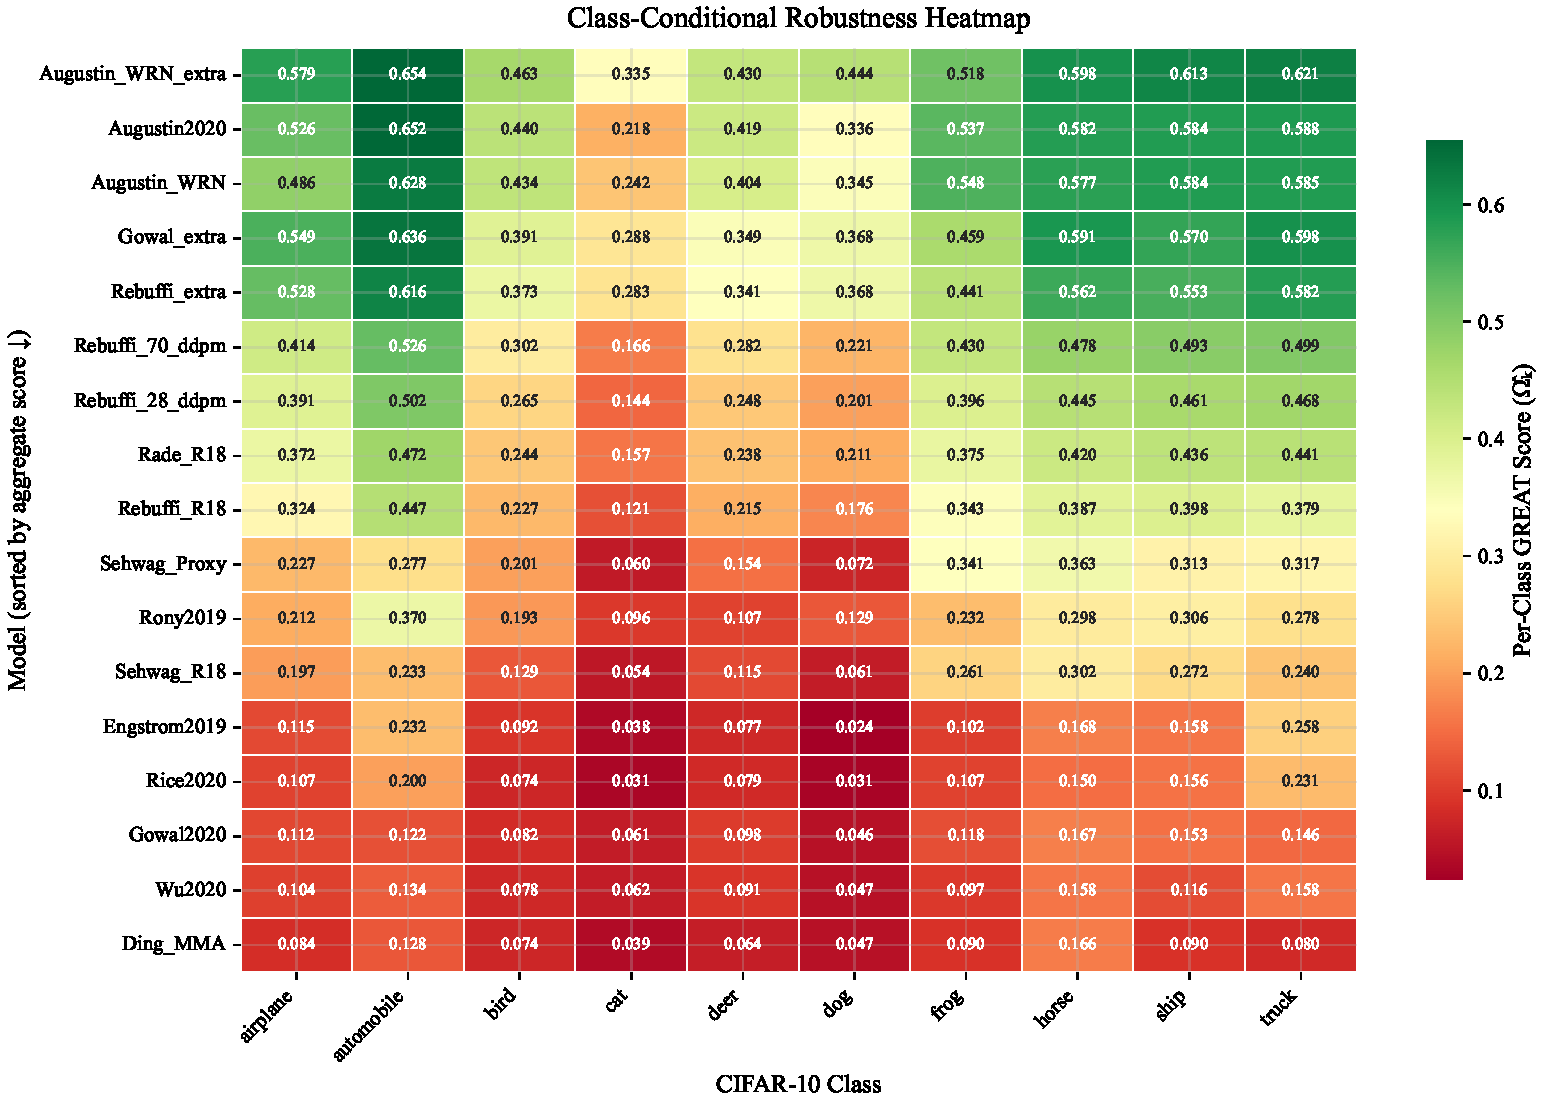
\includegraphics[width=\linewidth]{figures/cifar/heatmap.pdf}
    \caption{Per-class GREAT Scores for 17 CIFAR-10 models reveal substantial class-level robustness disparity hidden by aggregate scores. Each row is a model (sorted by aggregate GREAT Score); each column is a class. The class ``cat'' is consistently the most vulnerable (darkest column), while ``automobile'' is most often the most robust (10 of 17 models). Models with higher aggregate robustness (top rows) tend to exhibit \emph{greater} disparity between their strongest and weakest classes.}
    \label{fig:heatmap}
\end{figure}

In summary, we make the following contributions:
\begin{enumerate}
    \item We propose a \textbf{class-conditional decomposition} of the GREAT Score that preserves the certified lower-bound guarantee at per-class granularity, with formal concentration bounds (Propositions~\ref{prop:per_class_concentration} and~\ref{prop:rdi_concentration}).
    \item We introduce \textbf{four fairness-aware disparity metrics} (RDI, NRGC, WCR, FP-GREAT) grounded in welfare economics that quantify how robustness is distributed across classes.
    \item We propose an \textbf{attack-free self-calibration} procedure that replaces adversarial-attack-based temperature tuning with clean accuracy correlation, enabling fully attack-free evaluation.
    \item We conduct extensive experiments on \textbf{22 models across two benchmarks}, revealing consistent class vulnerability patterns and a quantifiable robustness-fairness tension that aggregate metrics conceal.
\end{enumerate}